\section{Benutzungsoberfläche}


\subsection{Sartfenster}

\begin{figure}[hp] 
  \centering
     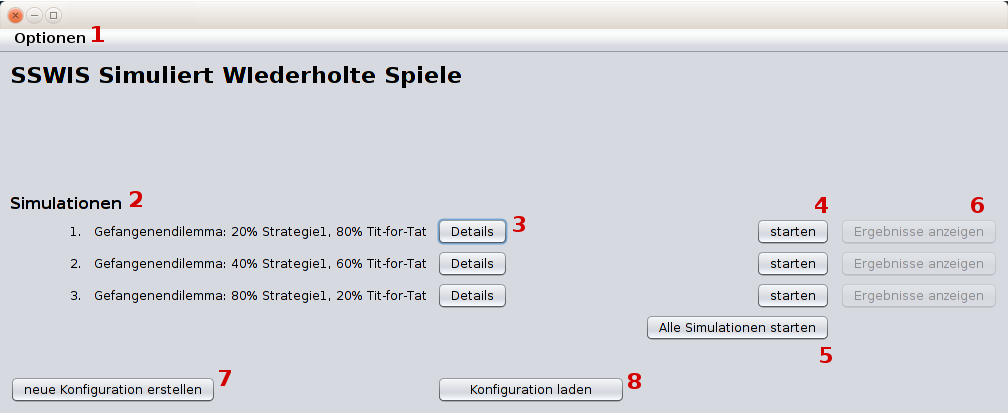
\includegraphics[width=1.2\textwidth]{GUI_Entwurf/StartfensterBeispiel.png}
  \caption{Entwurf}
  \label{fig:Bild1}
\end{figure}

\begin{description}


\item[1. Optionen] Menü enthält Zwei Untermenüs, Ergebnisse und Konfigurationen über die gespeicherte Ergebnisse und Startkonfigurationen angezeigt werden können

\item[2. Simulationen] Liste der geladenen Simulationen. Die wichtigsten Startkonfigurationen wie das Stufenspiel und die gewählten Strategien werden angezeigt.

\item[3. Details] Über diesen Knopf kann in einem Pop-Up-Fenster alle Parameter der Startkonfiguration eingesehen werden.

\item[4. starten] Die jeweilige Simulation kann über diesen Knopf ausgeführt werden. Wird die Simulation bereits ausgeführt oder ist sie in der Warteschlange, so ist der Knopf deaktiviert.

\item[5. Alle Simulationen starten] Durch diesen Knopf werden alle Simulationen, die nicht gerade ausgeführt oder bereits in der Warteschlange sind, nach einander ausgeführt. 

\item[6. Ergebnisse anzeigen] Bei Betätigung werden die Ergebnisse der jeweiligen Simulation der letzen Ausführung angezeigt. Wurde die Simulation noch nicht ausgeführt, ist der Knopf deaktiviert.

\item[7. neue Konfiguration erstellen] Führt zum Assistenten, um alle Parameter für eine neue Startkonfiguration zu bestimmen.

\item[8. Konfiguration laden] Öffnet ein Dialogfenster, in dem man eine zuvor gespeicherte Konfiguration auswählen kann.

\end{description}


\subsection{Konfigurationen erstellen}

\begin{figure}[hp] 
  \centering
     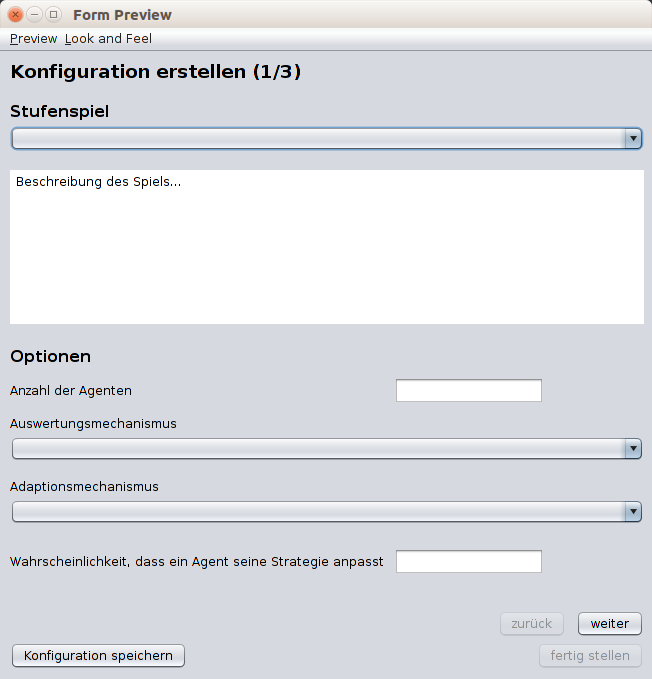
\includegraphics[width=1.0\textwidth]{GUI_Entwurf/WizardFenster1.png}
  \caption{Entwurf}
  \label{fig:Bild1}
\end{figure}

\begin{description}

\item[1. Stufenspiel] Es kann ein Stufenspiel gewählt werden

\item[2. Beschreibung des Spiels] Wenn ein Stufenspiel gewählt ist, steht hier eine kurze Beschreibung unteranderem mit den unterschiedlichen Auszahlungen

\item[3. Anzahl der Agenten] Es werden nur gerade Zahlen akzeptiert

\item[4. Auswertungsmechanismus] Es kann zwischen den Auswertungsmechanismen gewählt werden.

\item[5. Adaptionsmechanismus] Es kann zwischen den Adaptionsmechanismen gewählt werden.

\item[6. Wahrscheinlichkeit] Hier kann eine Wahrscheinlichkeit größer als null und kleiner gleich 100 in Prozent angegeben werden, dass Agenten nach einem Zyklus ihre Startegie gegebenen falls anpassen.

\item[7. Konfiguration speichern] Es öffnet sich ein Dialogfenster, um einen Namen für die erstellt Konfiguration zu bestimmen.

\item[8. zurück] Ist auf dieser Seite deaktiviert.

\item[9. weiter] Führt zur nächsten Seite, wenn alle Parameter korrekt eingegeben wurden. Bei falschen oder fehlenden Eingaben gibt es eine Fehlermeldung.

\item[10. fertig stellen] Ist aktiviert wenn alle nötigen Eingaben auf dieser und den anderen zwei Seiten getätigt wurden. Wenn alle Eingaben korrekt sind, wird das Fenster geschlossen und die Simulationen werden auf die Startseite geladen. Bei falschen oder fehlenden Eingaben gibt es eine Fehlermeldung.

\end{description}

\pagebreak

\begin{figure}[hp] 
  \centering
     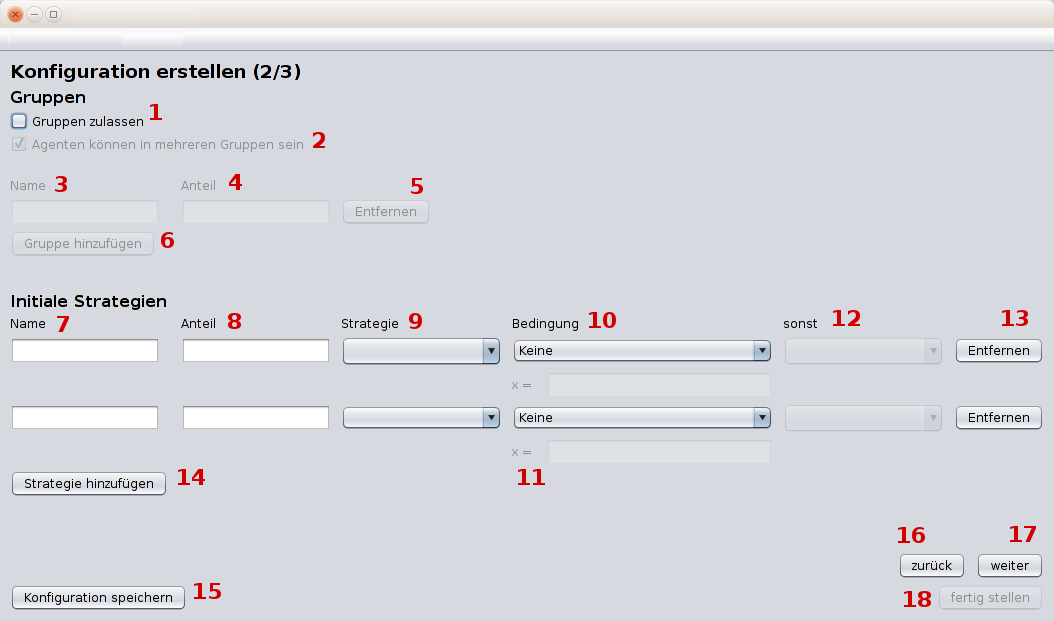
\includegraphics[width=1.2\textwidth]{GUI_Entwurf/WizardFenster2.png}
  \caption{Entwurf}
  \label{fig:Bild1}
\end{figure}

\begin{description}

\item[1. Gruppen zulassen] Aktiviert die Felder 2 bis 6 und aktiviert Bedingung die sich auf Gruppen beziehen.

\item[2. Agenten können in mehreren Gruppen sein] Lässt Überlappungen von Gruppen zu.

\item[3. Name] Name der Gruppe.

\item[4. Anteil] Anteil der Agenten in dieser Gruppe zu Beginn des Spiels in Prozent. Es werden Eingaben größer als null und kleiner gleich 100 akzeptiert.

\item[5. Entfernen] Es kann zwischen den Adaptionsmechanismen gewählt werden.

\item[6. Gruppe hinzufügen] Fügt eine neue Zeile mit den Feldern 3 bis 5 an.

\item[7. Name] Name der erstellten Strategie.

\item[8. Anteil] Anteil der Agenten in dieser Gruppe zu Beginn des Spiels in Prozent. Es werden Eingaben größer als null und kleiner gleich 100 akzeptiert. Alle Anteil-Felder müssen zusammen 100 ergeben.

\item[9. Strategie] Wähle zwischen vier 'Basis-Strategien': Tit-for-Tat, Grim, keine Kooperation, immer Kooperation

\item[10. Bedingung] Wähle die Bedingung mit der die Strategie eintritt. 

\item[11. x] Falls die Bedingung 'mit Wahrscheinlichkeit x' gewählt ist kann hier die Wahrscheinlichkeit in Prozent eingegeben werden. Die Eingabe muss dann größer als null und kleiner gleich 100 sein. Falls die Bedingung 'mit Gruppe x' gewählt ist kann hier der Name der Gruppe eingegeben werden. Sonst ist das Feld deaktiviert.

\item[12. sonst] Hier kann die alternative 'Basis-Strategien' gewählt werden, die eintritt, wenn die erste Strategie nicht eintritt.

\item[13. entfernen] Alle Felder in dieser Zeile werden gelöscht.

\item[14. Strategie hinzufügen] Fügt eine neue Zeile an, mit den Feldern 7 bis 13.

\item[15. Konfiguration speichern] Es öffnet sich ein Dialogfenster, um einen Namen für die erstellt Konfiguration zu bestimmen.

\item[16. zurück] Führt zu der ersten Seite.

\item[17. weiter] Führt zur nächsten Seite, wenn alle Parameter korrekt eingegeben wurden. Bei falschen oder fehlenden Eingaben gibt es eine Fehlermeldung.

\item[18. fertig stellen] Ist aktiviert wenn alle nötigen Eingaben auf dieser und den anderen zwei Seiten getätigt wurden. Wenn alle Eingaben korrekt sind, wird das Fenster geschlossen und die Simulationen werden auf die Startseite geladen. Bei falschen oder fehlenden Eingaben gibt es eine Fehlermeldung.

\end{description}

\pagebreak

\begin{figure}[hp] 
  \centering
     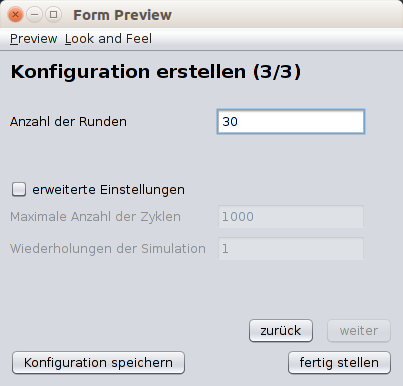
\includegraphics[width=0.7\textwidth]{GUI_Entwurf/WizardFenster3.png}
  \caption{Entwurf}
  \label{fig:Bild1}
\end{figure}

\begin{description}

\item[1. Anzahl der Runden] Die Anzahl der Runden in einer Simulation. Eine Runde besteht aus den Schritte Agenten miteinander paaren und Agenten spielen gegeneinander. Es werden ganzzahlige Eingaben akzeptiert.

\item[2. erweiterte Eintellungen] Nur wenn der Haken gesetzt ist, sind die unteren zwei Felder 3 und  aktiviert.

\item[3. Maximale Anzahl der Zyklen] Maximale Anzahl der Zyklen, nachdenen die Simulation abgebrochen wird, auch wenn kein Gleichgewichtszustand erreicht wurde. Ein Zyklus Besteht aus der angegebenen Anzahl von Runden und die darauffolgende Bewertung, der Agenten und die Anpassung ihrer Strategien. Es werden ganzzahlige Eingaben akzeptiert.

\item[4. Wiederholungen der Simulation] Anzahl der Wiederholungen der ganzen Simulation. Es werden ganzzahlige Eingaben akzeptiert.

\item[5. Konfiguration speichern] Es öffnet sich ein Dialogfenster, um einen Namen für die erstellt Konfiguration zu bestimmen.

\item[6. zurück] Führt zur zweiten Seite.

\item[7. weiter] Ist auf dieser Seite deaktiviert.

\item[8. fertig stellen] Ist aktiviert wenn alle nötigen Eingaben auf dieser und den anderen zwei Seiten getätigt wurden. Wenn alle Eingaben korrekt sind, wird das Fenster geschlossen und die Simulationen werden auf die Startseite geladen. Bei falschen oder fehlenden Eingaben gibt es eine Fehlermeldung.

\end{description}


\subsection{Konfigurationen speichern und laden}

\begin{figure}[hp] 
  \centering
     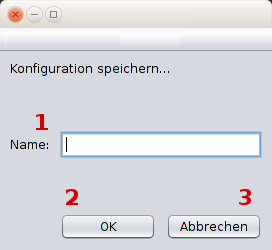
\includegraphics[width=0.5\textwidth]{GUI_Entwurf/KonfigSpeichern.png}
  \caption{Entwurf}
  \label{fig:Bild1}
\end{figure}

\begin{description}

\item[1. Name] Name für die zu speichernde Konfiguartion
\item[2. OK] Wurde ein Name eingegeben, so wird das Fenster geschlossen und alle durch den Assistenten eingegeben Parameter, der Startkonfiguration unter diesem Namen gespeichert.
\item[3. Abbrechen] Der Vorgang wird abgebrochen und das Fenster schließt sich.

\end{description}

\pagebreak

\begin{figure}[hp] 
  \centering
     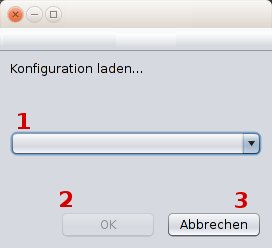
\includegraphics[width=0.5\textwidth]{GUI_Entwurf/KonfigLaden.png}
  \caption{Entwurf}
  \label{fig:Bild1}
\end{figure}

\begin{description}

\item[1. Konfiguration] Es kann zwischen den bereits gespeicherten Konfigurationen gewählt werden.
\item[2. OK] Wurde eine Konfiguration gewählt, so wird das Fenster geschlossen und der Assistent wird geöffnet. Alle gespeicherten Parameter der gewählten Konfiguration sind im Assistenten bereits eingegeben.
\item[3. Abbrechen] Der Vorgang wird abgebrochen und das Fenster schließt sich.

\end{description}

\pagebreak

\subsection{Ergebnisse anzeigen}

\begin{figure}[hp] 
  \centering
     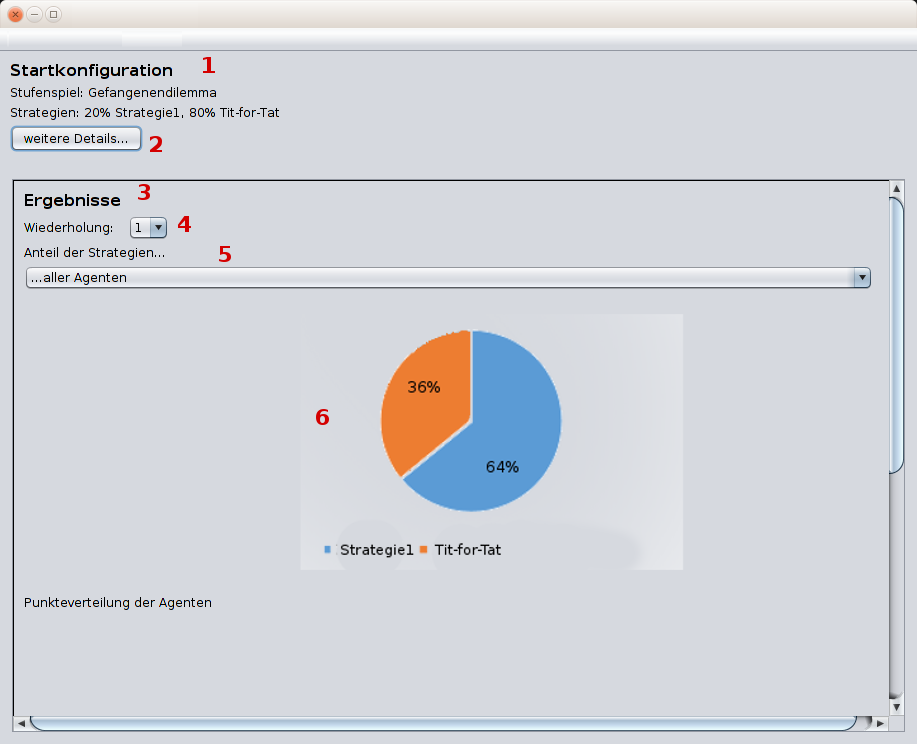
\includegraphics[width=1.2\textwidth]{GUI_Entwurf/Ergebnisfenster1.png}
  \caption{Entwurf}
  \label{fig:Bild1}
\end{figure}

\begin{description}

\item[1. Startkonfiguartion] Die wichtigsten Parameter der Startkonfiguration werden angezeigt.

\item[2. Details] In einem Pop-Up-Fenster werden alle Parameter der Startkonfiguration angezeigt.

\item[3. Ergebnisse] Das Feld zum anzeigen der Ergebnisse lässt sich scrollen.

\item[4. Wiederholung] Es kann zwischen den einzelnen Wiederholungen der Simulation gewählt werden. D

\item[5. Anteil der Strategien] Anteil der Strategien aller Agenten am Ende der Simulation. 

\item[6. zurück] Zeigt den Anteil der Strategien aller Agenten am Ende der Simulation in einem Kuchendiagramm. 

\end{description}

\pagebreak

\begin{figure}[hp] 
  \centering
     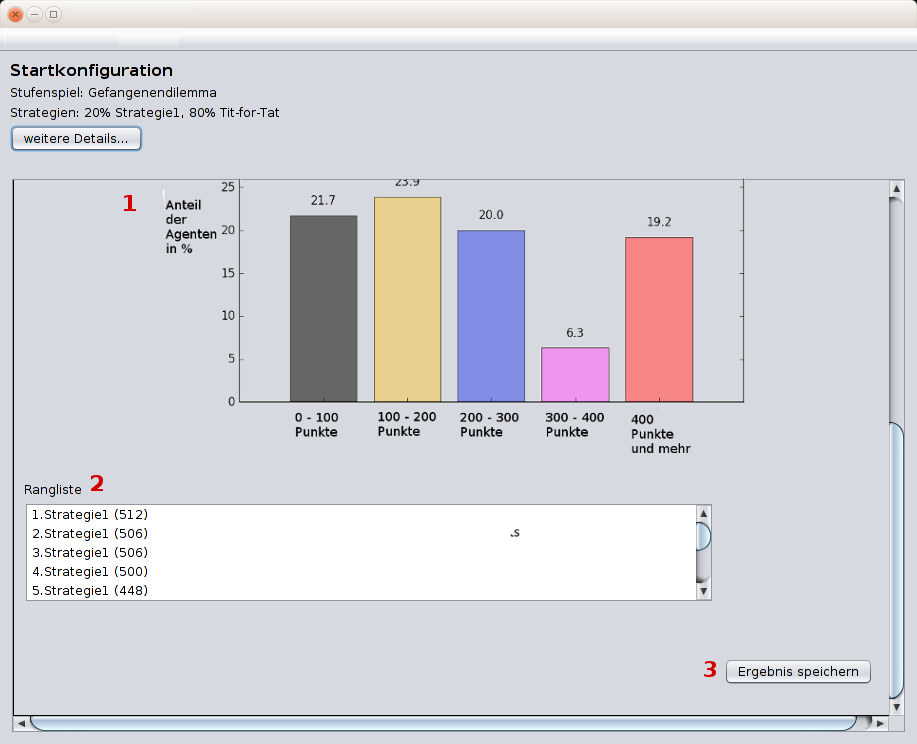
\includegraphics[width=1.2\textwidth]{GUI_Entwurf/Ergebnisfenster2.png}
  \caption{Entwurf}
  \label{fig:Bild1}
\end{figure}

\begin{description}

\item[1. Punkteverteilung der Agenten] Zeigt die Verteilung der Summe aller Auszahlungen der Agenten am Ende der Simulation in einem Balkendiagramm an.

\item[2. Rangliste] Zeigt eine Rangliste aller Agenten am Ende der Simulation mit ihrem Rang ihre letzten Strategie und die Summe aller ihrer Auszahlungen.

\item[3. Ergebnisse speichern] Öffnet ein Dialogfenster in den ein Name für die Ergebnisse gewählt werden kann.


\end{description}


